% \part{Projeto}

\chapter[Projeto]{Projeto}

\section{Requisitos}

Para o desenvolvimento do projeto de uma arquitetura de Data Fabric para salvar imagens de câncer de pele, foram definidos os seguintes requisitos:

\subsection{Requisitos Funcionais}
\begin{table}[H]
    \centering
    \begin{tabular}{|c|p{12cm}|}
    \hline
    \textbf{ID} & \textbf{Requisito} \\ \hline
    RFSO01 & O sistema deve ser capaz de armazenar grandes volumes de imagens de câncer de pele. \\ \hline
    RFSO02 & O sistema deve permitir o processamento eficiente das imagens armazenadas. \\ \hline
    RFSO03 & O sistema deve garantir a segurança e a privacidade dos dados dos pacientes. \\ \hline
    RFSO04 & Os dados devem estar disponíveis para acesso por pesquisadores e profissionais de saúde de forma segura. \\ \hline
    RFSO05 & O sistema deve ser escalável para acomodar o aumento no volume de dados ao longo do tempo. \\ \hline
    RFSO06 & O sistema deve permitir o compartilhamento seguro de dados utilizando Delta Sharing. \\ \hline
    RFSO07 & O sistema deve permitir a integração de dados de diferentes fontes de forma unificada. \\ \hline
    RFSO08 & O sistema deve oferecer uma camada de virtualização para consulta de dados distribuídos. \\ \hline
    RFSO09 & O sistema deve permitir a governança centralizada dos dados, com controle de acesso baseado em papéis. \\ \hline
    RFSO10 & O sistema deve suportar análises em tempo real para dados armazenados e em trânsito. \\ \hline
    RFSO11 & O sistema deve possuir uma camada de metadados para catalogação de imagens e dados relacionados. \\ \hline
    RFSO12 & O sistema deve fornecer APIs para facilitar a integração com ferramentas de visualização de dados. \\ \hline
    \end{tabular}
    \caption{Tabela de Requisitos Funcionais}
    \label{tab:requisitos_funcionais}
\end{table}

\subsection{Requisitos Não Funcionais}
\begin{table}[H]
    \centering
    \begin{tabular}{|c|p{12cm}|}
    \hline
    \textbf{ID} & \textbf{Requisito} \\ \hline
    RNFSO01 & O sistema deve ser capaz de processar e recuperar dados rapidamente. \\ \hline
    RNFSO02 & O sistema deve garantir a integridade e a consistência dos dados armazenados. \\ \hline
    RNFSO03 & A interface do sistema deve ser intuitiva e fácil de usar para os profissionais de saúde. \\ \hline
    RNFSO04 & O sistema deve ser de fácil manutenção e atualização. \\ \hline
    RNFSO05 & A arquitetura deve ser modular para facilitar a expansão e substituição de componentes. \\ \hline
    RNFSO06 & O sistema deve oferecer suporte a padrões de interoperabilidade, como FHIR. \\ \hline
    RNFSO07 & O sistema deve garantir compatibilidade com regulamentações de proteção de dados, como LGPD. \\ \hline

    \end{tabular}
    \caption{Tabela de Requisitos Não Funcionais}
    \label{tab:requisitos_nao_funcionais}
\end{table}

\subsection{Histórias de Usuário}
\begin{table}[H]
    \centering
    \begin{tabular}{|c|p{8cm}|c|c|}
    \hline
    \textbf{Requisitos} & \textbf{Descrição} & \textbf{MoSCoW} & \textbf{Pontuação} \\ \hline
    RFSO01 & Como pesquisador, quero armazenar grandes volumes de imagens de câncer de pele para análise. & Must Have & 8 \\ \hline
    RFSO03 & Como administrador, quero garantir a privacidade dos dados dos pacientes armazenados. & Must Have & 9 \\ \hline
    RFSO04 & Como médico, quero acessar dados de forma segura para apoiar o diagnóstico. & Must Have & 8 \\ \hline
    RFSO06 & Como pesquisador, quero compartilhar dados de forma segura com outras organizações ou contribuidores. & Should Have & 7 \\ \hline
    RFSO07 & Como administrador, quero integrar dados de diferentes bases de dados para análise centralizada. & Must Have & 9 \\ \hline
    RFSO08 & Como pesquisador, quero consultar dados distribuídos sem me preocupar com a origem física dos dados. & Should Have & 7 \\ \hline
    RFSO09 & Como administrador, quero controlar acessos de forma centralizada para garantir segurança. & Must Have & 8 \\ \hline
    RFSO10 & Como pesquisador, quero realizar análises em tempo real para melhorar a precisão dos resultados. & Could Have & 6 \\ \hline
    RFSO11 & Como desenvolvedor, quero acessar um catálogo centralizado de metadados para identificar rapidamente os dados necessários. & Should Have & 7 \\ \hline
    RNFSO07 & Como administrador, quero garantir que os dados do sistema estejam em conformidade com LGPD. & Must Have & 10 \\ \hline
    \end{tabular}
    \caption{Tabela de Histórias de Usuário}
    \label{tab:historias_usuario}
\end{table}

\section{Arquitetura}

A arquitetura do projeto será baseada na abordagem de Data Fabric, que permite a integração e gestão de dados de forma unificada e eficiente. A seguir, a descrição dos principais componentes da arquitetura:

\subsection{Diagrama de Arquitetura}
O diagrama a seguir ilustra a arquitetura do sistema:
\begin{figure}[h]
    \centering
    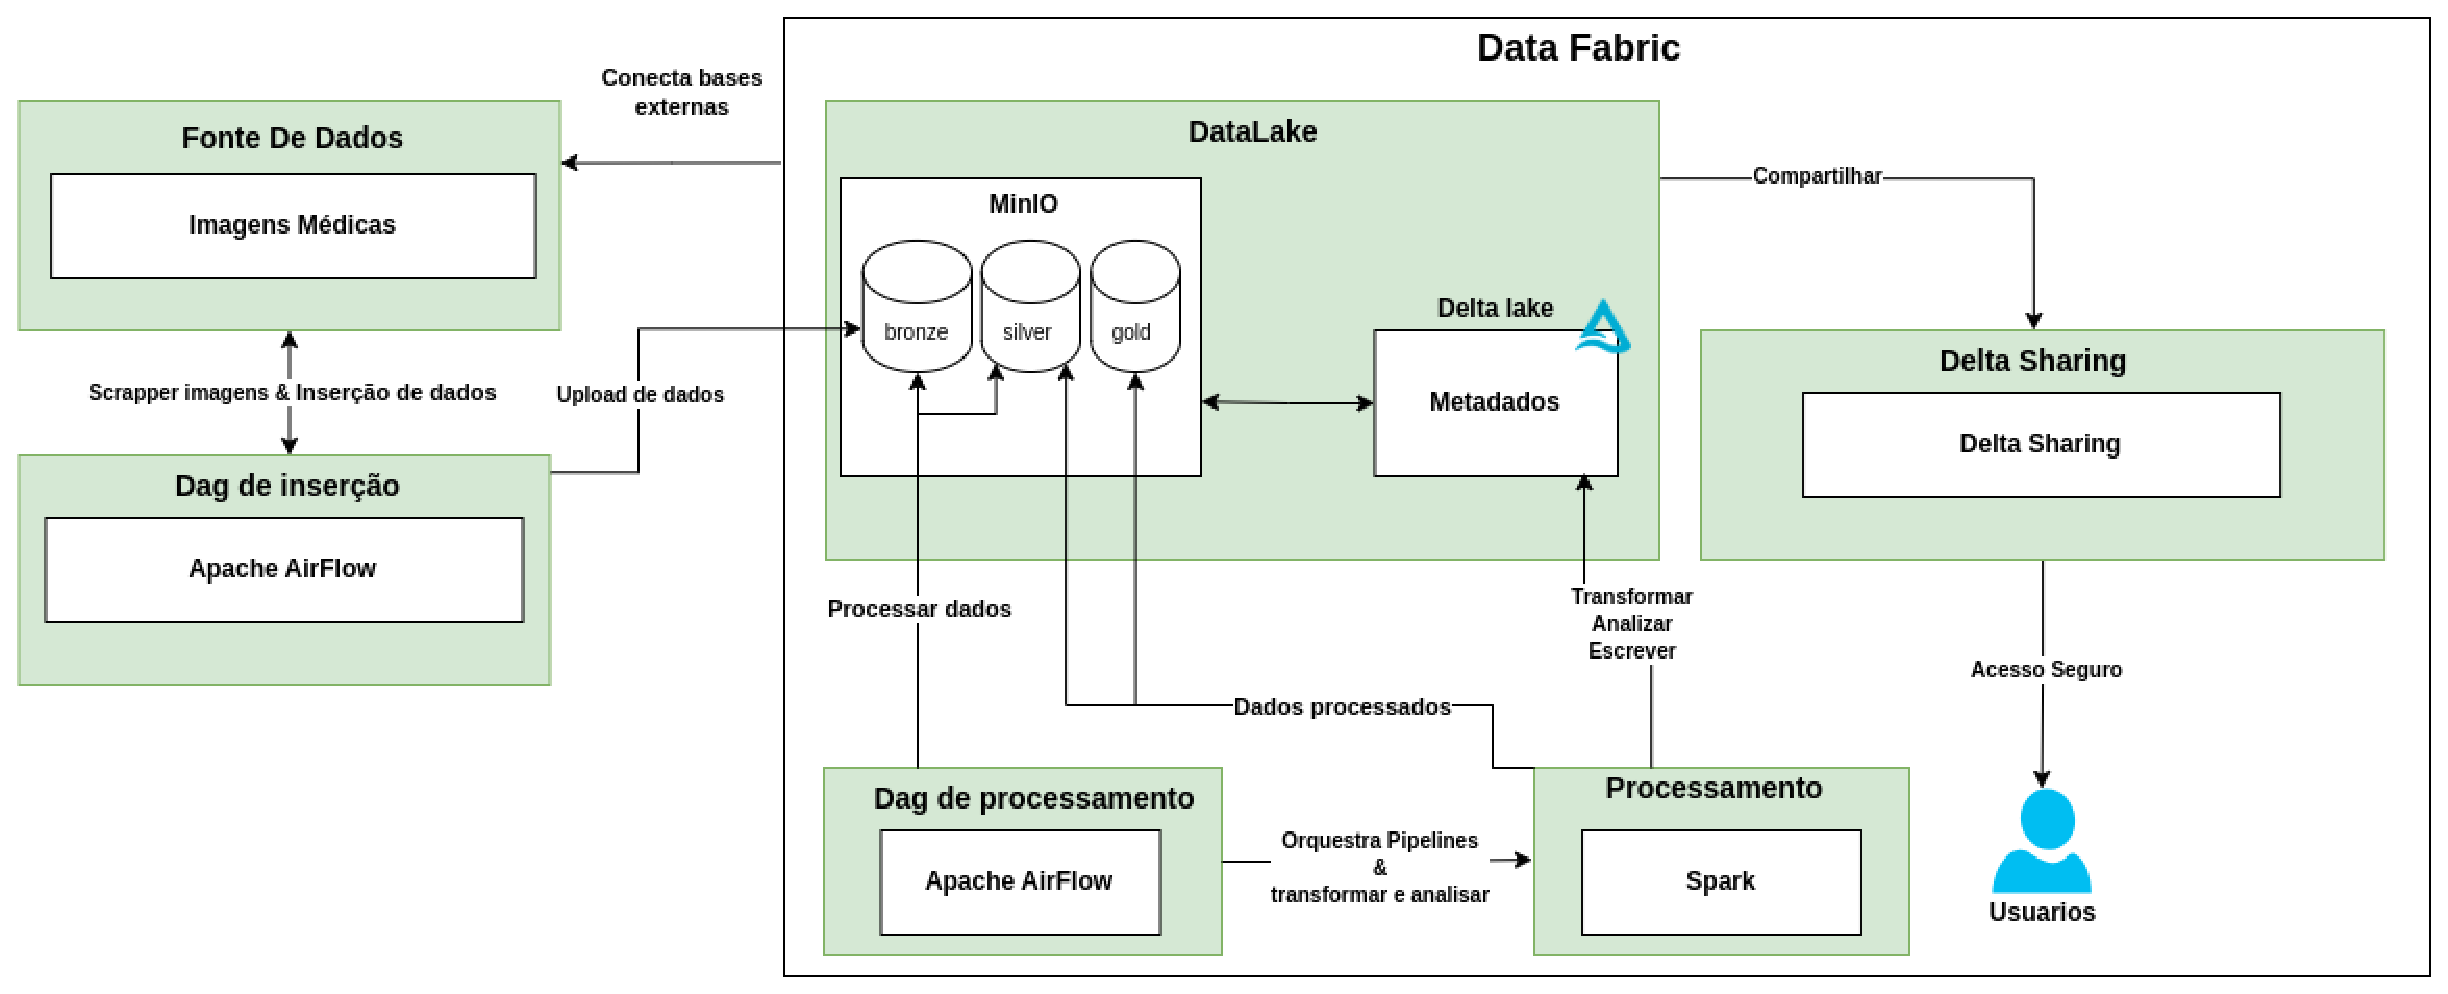
\includegraphics[width=0.8\textwidth]{figuras/arquitetura.eps}
    \caption{Diagrama da Arquitetura do Projeto }
    \label{fig:arquitetura_projeto}
\end{figure} 



\subsection{Componentes da Arquitetura}
\begin{itemize}
    \item \textbf{Ingestão de Dados}: Utilização de pipelines de ingestão para coletar e armazenar imagens de câncer de pele de diversas fontes (hospitais, clínicas, pesquisas).
    \item \textbf{Armazenamento de Dados}: Implementação de um sistema de armazenamento distribuído, como MinIO, para garantir a escalabilidade e a disponibilidade das imagens.
    \item \textbf{Processamento de Dados}: Utilização de ferramentas como Apache Airflow para a orquestração de pipelines de processamento das imagens.
    \item \textbf{Gestão de Dados}: Aplicação de Data Fabric para fornecer uma camada de abstração que facilita a integração e gestão dos dados distribuídos.
    \item \textbf{Compartilhamento de Dados}: Utilização de Delta Sharing para permitir o compartilhamento seguro de dados entre diferentes organizações.
    \item \textbf{Interface de Usuário}: Desenvolvimento de uma interface web utilizando FastAPI para permitir o acesso e a manipulação dos dados por pesquisadores e profissionais de saúde.
\end{itemize}

\subsection{Fluxo de Dados}
\begin{itemize}
    \item \textbf{Coleta e Ingestão}: As imagens são coletadas de diversas fontes e armazenadas no sistema de armazenamento distribuído.
    \item \textbf{Processamento}: As imagens armazenadas são processadas através de pipelines orquestrados pelo Apache Airflow, que podem incluir etapas de pré-processamento, análise e extração de características.
    \item \textbf{Armazenamento e Gestão}: Os dados processados são armazenados e geridos pela arquitetura de Data Fabric, que garante a integração e a consistência dos dados.
    \item \textbf{Compartilhamento de Dados}: Utilizando Delta Sharing, os dados podem ser compartilhados de forma segura com outras organizações e pesquisadores.
    \item \textbf{Acesso aos Dados}: A interface web desenvolvida com FastAPI permite que os usuários acessem e manipulem os dados de forma segura e eficiente.
\end{itemize}

\section{Tecnologias Utilizadas}

Com base no referencial teórico, as seguintes tecnologias serão utilizadas no projeto:
\begin{itemize}
    \item \textbf{MinIO}: Para o armazenamento distribuído das imagens, garantindo escalabilidade e disponibilidade.
    \item \textbf{Apache Airflow}: Para a orquestração de pipelines de processamento de dados.
    \item \textbf{Data Fabric}: Para a integração e gestão de dados de forma unificada.
    \item \textbf{Delta Sharing}: Para o compartilhamento seguro de dados entre diferentes organizações.
    \item \textbf{FastAPI}: Para o desenvolvimento da interface web, permitindo o acesso e a manipulação dos dados.
    \item \textbf{Kubernetes}: Para a orquestração de containers, garantindo a escalabilidade e a alta disponibilidade do sistema.
    \item \textbf{Spark}: Fornece um alto nível de paralelismo, processando grandes quantidades de dados eficientimente em vários nós em um cluster.
\end{itemize}

\section{Conclusão}

O projeto visa implementar uma arquitetura robusta e escalável de Data Fabric para o armazenamento e processamento de imagens de câncer de pele. A utilização das tecnologias mencionadas, incluindo Delta Sharing, garantirá a segurança, a eficiência e a acessibilidade dos dados, contribuindo significativamente para a pesquisa e o diagnóstico médico.